
\documentclass[a4paper, 12pt]{report}
\usepackage[T1]{fontenc}
\usepackage[utf8]{inputenc} % FIXME maybe 
\usepackage{placeins}
\usepackage[top=2.2cm, bottom=2.2cm, left=2.0cm, right=2.0cm]{geometry} % margins
\usepackage[justification=centering]{caption}
\captionsetup[table]{name=Tab.}
\usepackage[englishb]{babel} %language
\usepackage{graphicx} % support the \includegraphics command and options
\usepackage{color}    %colorful text
\usepackage{ulem}
\usepackage{steinmetz} % permet d'utiliser \phase{}
\usepackage{gensymb} % permet d'utiliser le symbole ° avec \degree
\usepackage{colortbl} % permet de colorer des cellules de tableaux
\definecolor{lightgray}{gray}{0.85} % création couleur gris clair
\usepackage[toc,page]{appendix} % ajouté par moi : permet l'utilisation de la commande \begin{appendices} pour faire les annexes
\renewcommand{\appendixpagename}{Annexes} % pour afficher Annexes en français
\renewcommand{\appendixtocname}{Annexes} % pour afficher Annexes en français
\usepackage{multirow} % permet de fusionner des cellules d'un tableau
\usepackage{diagbox} % permet d'utiliser la commande \diagbox pour diviser diagonalement une cellule d'un tableau
\usepackage{chemfig}
\usepackage{hhline}
\usepackage{eurosym}
\definecolor{mygreen}{RGB}{28,172,0} % color values Red, Green, Blue
\definecolor{mylilas}{RGB}{170,55,241}
\usepackage{amsmath, amssymb}  % for better maths
\usepackage{bbold}
\usepackage{booktabs} % for much better looking tables
\usepackage{array}    % for better arrays (eg matrices) in maths
\usepackage{paralist} % very flexible & customisable lists (eg. enumerate/itemize, etc.)
\usepackage{verbatim} % adds environment for commenting out blocks of text & for better verbatim
\usepackage{subfig}   % make it possible to include more than one captioned figure/table in a single float
\usepackage{eurosym}
\usepackage{subfigure}
\usepackage{subfig}
\usepackage{subcaption}
\usepackage{float}
\usepackage{appendix}
\renewcommand{\thesection}{\arabic{section}}
\setcounter{secnumdepth}{3}
\renewcommand{\figurename}{\textsc{Figure}}

% Table of Contents' look
\usepackage[nottoc,notlof,notlot]{tocbibind}   % Put the bibliography in the ToC (table of contents)
\usepackage[titles,subfigure]{tocloft}         % Alter the style of the Table of Contents
\renewcommand{\cftsecfont}{\rmfamily\mdseries\upshape}
\renewcommand{\cftsecpagefont}{\rmfamily\mdseries\upshape} % No bold!

% These packages will all be used one day or another...
\usepackage{tabularx}
\usepackage[hyphens]{url} % option hyphnens to break the url into multiple lines if needed
\usepackage[colorlinks=true,urlcolor=cyan,linkcolor= blue]{hyperref}
%\usepackage{fullpage}
\usepackage{epstopdf}
% Be able to include some source code! 
\usepackage{listings} % pour insérer du code
\usepackage{bm} % avoir les lettre grecques en gras


\lstset{language=Matlab,%
    %basicstyle=\color{red},
    breaklines=true,%
    morekeywords={matlab2tikz},
    keywordstyle=\color{blue},%
    morekeywords=[2]{1}, keywordstyle=[2]{\color{black}},
    identifierstyle=\color{black},%
    stringstyle=\color{mylilas},
    commentstyle=\color{mygreen},%
    showstringspaces=false,%without this there will be a symbol in the places where there is a space
    numbers=left,%
    numberstyle={\tiny \color{black}},% size of the numbers
    numbersep=9pt, % this defines how far the numbers are from the text
    emph=[1]{for,end,break},emphstyle=[1]\color{red}, %some words to emphasise
    %emph=[2]{word1,word2}, emphstyle=[2]{style},    
}

\usepackage[export]{adjustbox}

\lstset{commentstyle=\color{red},keywordstyle=\color{black},
showstringspaces=false}
\lstnewenvironment{rc}[1][]{\lstset{language=R}}{}
\newcommand{\ri}[1]{\lstinline{#1}}  %% Short for 'R inline'
\usepackage{fancyhdr}
\pagestyle{fancy}
\renewcommand{\sectionmark}[1]{\markboth{\thesection.\ #1}{}}
\lstset{language=R} % Set R to default language.


\lfoot{\footnotesize University of Liège}
\cfoot{\footnotesize -\space\thepage\space-}
\rfoot{\footnotesize Machine learning}
\renewcommand{\headrulewidth}{0.4pt}
\renewcommand{\footrulewidth}{0.4pt}

\renewcommand{\bf }{\mathbf}
\newcommand{\Biais}{\textcolor{teal}{\textbf{Biais }}}
\newcommand{\biais}{\textcolor{teal}{\textbf{biais }}}
\newcommand{\variance }{\textcolor{red}{\textbf{variance }}}
\newcommand{\Variance }{\textcolor{red}{\textbf{Variance }}}
\newcommand{\noise }{\textcolor{blue}{\textbf{noise }}}
\newcommand{\reglin }{\textbf{regression linéaire }}
\newcommand{\linreg }{\textbf{linear regression }}
\newcommand{\regtr }{\textbf{Regression Trees }}
\definecolor{ao}{rgb}{0.0, 0.5, 0.0}
\definecolor{red.g}{rgb}{0.91, 0.29, 0.27}
\definecolor{blue.g}{rgb}{0.2, 0.75, 0.89}
\definecolor{vert.g}{rgb}{0.58, 0.96, 0.51}
\newcommand{\algo }{\textbf{algorithm}}
\newcommand{\example}{\textcolor{ao}{\textbf{example }}}
\newcommand{\Example}{\textcolor{ao}{\textbf{Example }}}
\newcommand{\exemple}{\textcolor{ao}{\textbf{exemple }}}
\newcommand{\Exemple}{\textcolor{ao}{\textbf{Exemple }}}

\newcommand{\Advantages}{\textcolor{ao}{\textcolor{ao}{\textbf{Advantages }}}}
\newcommand{\Drawbacks}{\textcolor{red}{\textcolor{ao}{\textbf{Drawbacks}}}}


\date{\today}

%-------------------------------------------------------------
%                 OPTION D'INSERTION DE CODE.
%-------------------------------------------------------------
\definecolor{mygreen}{rgb}{0,0.6,0}
\definecolor{mygray}{rgb}{0.5,0.5,0.5}
\definecolor{mymauve}{rgb}{0.58,0,0.82}

\lstset{ 
  backgroundcolor=\color{white},
  basicstyle=\footnotesize,
  breakatwhitespace=false,
  breaklines=true,
  captionpos=b,
  commentstyle=\color{mygreen},
  deletekeywords={...},            
  escapeinside={\%*}{*)},
  extendedchars=true,
  frameround= t t t t,
  keepspaces=true,
  keywordstyle=\color{blue},
  language=Matlab,
  otherkeywords={*,switch, case, otherwise},
  numbers=left,
  numbersep=5pt,
  numberstyle=\tiny\color{mygray},
  rulecolor=\color{black},
  showspaces=false,
  showstringspaces=false,
  showtabs=false,
  stepnumber=1,
  stringstyle=\color{mymauve},
  tabsize=2,
  xleftmargin = 5pt,
  inputpath = Functions
}

\usepackage{amsfonts}
\usepackage{amssymb}
\usepackage{amsmath}
\usepackage{amsthm}
\usepackage{enumitem}

\usepackage{bbold}
\usepackage{bm}
\usepackage{graphicx}
\usepackage{color}
\usepackage{hyperref}

\usepackage{indentfirst}
%-------------------------------------------------------------
%               FIN OPTION D'INSERTION DE CODE.
%-------------------------------------------------------------

\newcommand{\q}{\tilde{q}}
\newcommand{\qv}{\mathbf{q_v}}
\newcommand{\qvt}{\mathbf{\q_v}}
\newcommand{\matlab}{\textsc{Matlab }}
\newcommand{\vars}[1]{\textbf{\textcolor{blue}{#1}}}
\usepackage{newunicodechar}
\newcommand{\ct}{\textbf{Classification Trees}}
\newcommand{\Dt}{\textbf{Decision trees}}
\newcommand{\dt}{\textbf{decision trees}}
\newcommand{\rt}{\textbf{regression trees}}
\newcommand{\Rt}{\textbf{Regression trees}}
\newcommand\Warning{%
 \makebox[1.4em][c]{%
 \makebox[0pt][c]{\raisebox{.1em}{\small!}}%
 \makebox[0pt][c]{\color{red}\Large$\bigtriangleup$}}}%

\newunicodechar{⚠}{\Warning}
\usepackage{multicol}
\newcommand{\esp}{\text{ }}

\usepackage{tikz}


\begin{document}


\begin{titlepage}
	\begin{center}
	%
	~~\\
		% ~~\\
		 % ~~\\
		 
		
		{\fontsize{20}{20}\selectfont
		\textsc{ELEN062-1} \\
		%\vspace{0.5cm}
		
		\textsc{Machine learning }\\
		\vspace{0.3cm}
	    Pierre Geurts and Louis Wehenkel
		\vspace{2cm}
		
	\begin{figure}
	    \centering
	    
\includegraphics[width=16cm]{entete.png} 
	\end{figure}
	
	
	
		
    %\begin{figure} 
    %\begin{minipage}[l]{.46\linewidth}
    %    \includegraphics[width=7cm, left]{ulg.jpg}
    %\end{minipage} 
    %\begin{minipage}[r]{.46\linewidth}
    %    \includegraphics[width=5cm, right]{facsa.png}
    %\end{minipage}
    %\end{figure}

		\vspace{0.1cm}
		
		\hrulefill
		
		\vspace{0.2cm}
		{\fontsize{30}{25}\selectfont \textbf{Synthèses}\\}
		\vspace{0.2cm}
		
		
		% chiffre 1 : taille, chiffre 2 : interligne

		\hrulefill

		\vspace{1cm}
~~\\
		{\fontsize{20}{25}\selectfont
		Hubar Julien \\
		\vspace{3.1cm}
		\textit{Master 1 Data science Engineering}\\
		\textit{Faculty of Applied Sciences}
	   	
	  \vspace{2cm}
	  
		Academic years 2019-2020}
		}
	\end{center}

\end{titlepage}

%%%%%%%%%%%%%%%%%%%%%%%%%%%%%%%%%%%
%%%%%%%%%%%%%%%%%%%%%%%%%%%%%%%%%%%
% Début document
%%%%%%%%%%%%%%%%%%%%%%%%%%%%%%%%%%%
%%%%%%%%%%%%%%%%%%%%%%%%%%%%%%%%%%%
\tableofcontents
\newpage
\section{Machine learning protocols}
\subsection{Apprentissage supervisé}
L'apprentissage supervisé est une technique d'apprentissage \textcolor{blue}{\textbf{automatique}} où l'on cherhcer à produire \textbf{automatiquement des règles} à partir d'une base de données contenant des examples déjà traités. Le but de la méthode est de déterminer une représentation compacte de la base de données par une fonction dite de prédiction associant à une entrée, une sortie.\\
\Exemple: KNN, decision tree, Neural network. \\
\textbf{Application}: reconnaissance d'image, ou plus récemment la suppresion d'objet dans une image(application dans photoshope). 
\begin{figure}[H]
    \centering
    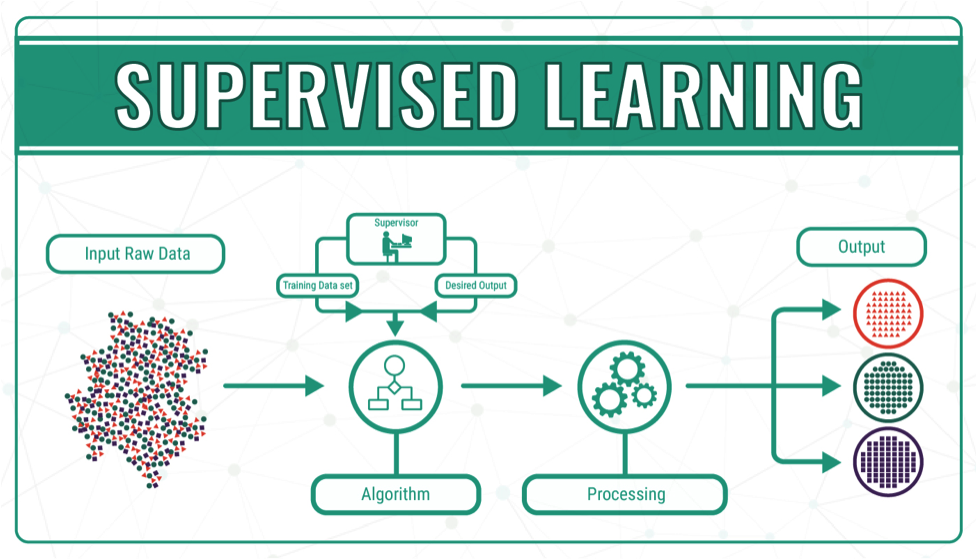
\includegraphics[scale = 0.5]{Question1/supervised-learning.png}
    \caption{}
    \label{fig:my_label}
\end{figure}
\subsection{Apprentissage non-supervisé}
L'apprentissage \textbf{non supervisé} est un problème d'apprentissage automatique. Il s'agit de trouver des stuctures sous-jacentes à partir de donnée \textbf{non} étiquetées. Puisque les données ne sont pas étiquetées, il n'est pas possible d'affecter  au résultat de l'algorithme utilisé un score d'adéquation. Cette absence d'étiquetage(ou d'annotation) est ce qui distingue les taches d'apprentissage non-supervisé des tâches d'apprentissage supervisé.
\begin{figure}[H]
    \centering
    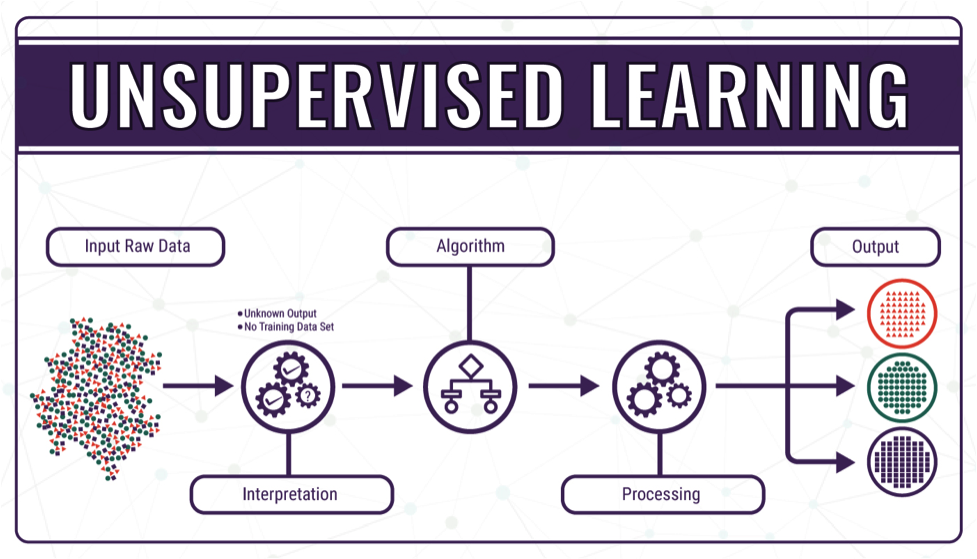
\includegraphics[scale = 0.5]{Question1/unsupervised-learning.png}
    \caption{}
    \label{fig:my_label}
\end{figure}

\subsection{Apprentisage non-supervisé vs. supervisé}
On distingue l'apprentissage supervisé et non supervisé. Dans le permier cas, il s'agit d'apprendre à classer un nouvel individu parmi un ensemble de classes prédéfinies: on connait les classes à priori. Tandis que dans l'apprentissage non supervisé, le nombre et la définition des classes ne sont pas donnés à priori.

\subsection{Apprentissage par renforcement}
L'apprentissagr par renforcement fait référence à une classe de problémes d'apprentissage automatique à partir d'expériences de façons à optimiser une récompense numérique au cours du temps. Un agent autonome, plongé au sein d'un environnement, cherche au travers d'expériences itérés un comportement décisionnel optimal, une politique (fonction) associant sont état courant à l'action à exécuter permettant de maximiser la somme des récompenses au cours du temps.

\begin{figure}[H]
    \centering
    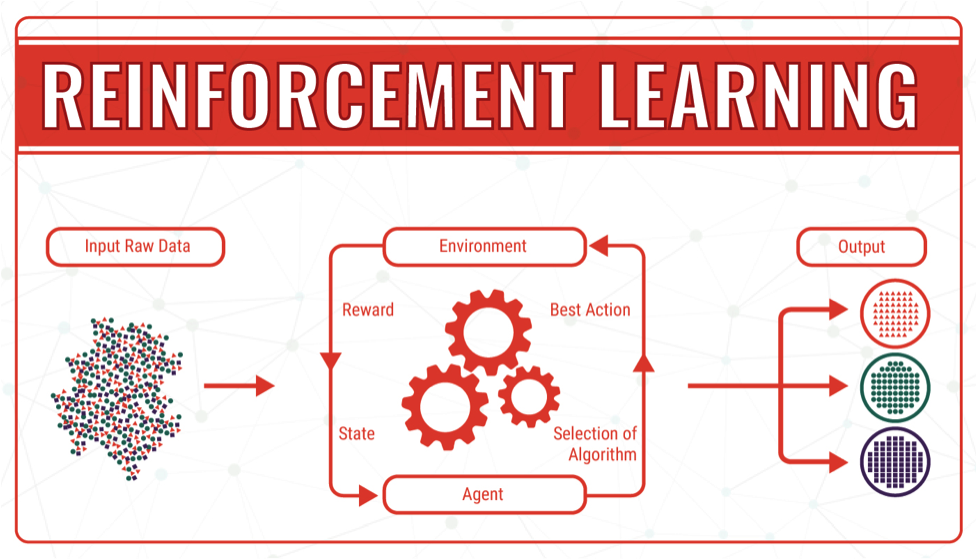
\includegraphics[scale = 0.25]{Question1/reinforcement-learning.png}
    \caption{}
    \label{fig:my_label}
\end{figure}
\subsubsection{Apprentissage en mode hors line (batch)}
\textcolor{red}{\textbf{Il exploite un max la DB}}\\
L'apprentissage en mode hos ligne(ou \textbf{batch}) est un cas particulier du reinforcement learning, qui est une classe de problèmes d'apprentisage dont l'obejectif est de déterminer à partir d'expériences une stratégie (ou politique) permettant à un agent de maximiser une récompense numérique au cours du temps.\\
Dans le cadre de l'apprentissage par renforcement purement hors ligne, l'agent ne peut interagir avec l'environnement: une base d'apprentissage lui est fournie au départ et il l'exploite pour apprendre une politique.\\\\
\textbf{Compément d'information}\\\\
Contrastant avec les algorithmes en-ligne, où l'agent à la possibilité d'interagir comme bon lui semble avec l'environnement, les algorithmes hors-ligne tentent d'exploiter au maximum les exemples d'apprentissage dont ils disposent, sans compter uniquement sur la possibilité d'exploration. Cette approche est donc particulièrement avantageuse quand il n'est pas possible d'effectuer des expériences ou lorsque ces expériences sont coûteuses (casse de matériel possible, obligation d'avoir recours à une assistance humaine pendant les expériences, etc). En général cependant, les techniques d'apprentissage par renforcement batch peuvent être utilisées

\subsubsection{Apprentissage en mode batch vs. apprentissage en mode on-line}
\begin{itemize}
    \item En mode \textbf{batch}, les échantillons sont fournis et calculés ensemble pour former le modèle alors qu'en mode on-line, les échantillons sont données un à un pour mettre à jour le modèle.
    \item E mode \textbf{batch}, les échantillons sont stockés et non le modèle, tandis qu'en mode on-line c'est le modèle qui est stocké et non les échantilons. 
    \item Le mode batch est une approche classique du data-mining alors que le mode \textbf{on-line} est une methode approche pour les systèmes adaptatifs.
\end{itemize}
Les deux mode peuvent êtrre adapté pour répondre à un même problème: pour des échantillons donnée, on peut les exploiter un par un pour obtenir un mode on-line,ainsi que, pour des échantillons donnée un par un on peut les stocker avant de les exploiter tous ensemble.\\
\textbf{Exemple: Reconnaissance de symboles manuscrits}
\\\\
\textbf{Complément d'information}\\\\
L’exploration de données, connue aussi sous l'expression de fouille de données, forage de données, prospection de données, \textbf{data mining}, ou encore extraction de connaissances à partir de données, a pour objet l’extraction d'un savoir ou d'une connaissance à partir de grandes quantités de données, par des méthodes automatiques ou semi-automatiques.
Elle se propose d'utiliser un ensemble d'algorithmes issus de disciplines scientifiques diverses telles que les statistiques, l'intelligence artificielle ou l'informatique, pour construire des modèles à partir des données, c'est-à-dire trouver des structures intéressantes ou des motifs selon des critères fixés au préalable, et d'en extraire un maximum de connaissances.
\subsection{Apprentissage semi-supervisé}
Le but de cet apprentissage est d'exploiter à la fois des données labélisées et celles qui ne le sont pas pour construire de meilleurs modèles que si on n'utilisait qu'un seul typde de données.\\
Différentes approches sont possibles : 
\begin{itemize}
    \item \textbf{SVM} semi-supervisé: énumérer toutes les labelisations possible (pour les données non labélisées), apprendre un SVM pour chacune et ne garder que celle avec la plus grande marge d'erreur. 
    \item Algo basé sur les graphes: Construire un graphe sur base des données des 2 types et apprendre un modèles qui prédit correctement les données et qui lisse le graphe.
\end{itemize}
\textbf{Exemple}: Diagnostique médical par \textbf{SVM}
\subsection{Apprentissage transductif}
Semblable à l'apprentissage supervisé mais on a accès dès le début aux données de test qu'on veut utiliser sans construire de modèle pour calculer les prédictions des données non labélisées.\\
\textbf{Solution simple}: appliquer des techniques d'apprentissage semi-supervisé en utilisant des données de test comme données non labélisées pour obtenir un modèle qui servira à prédire les données de test.

\section{Model evalution criteria}
\subsection{Error rate}
Build contagency table recording the number of TN,TP,FP,FN
  \begin{table}[!h]
    \begin{center}
    \begin{tabular}{| m{5em}| m{5em}|}
    \hline
    \centering
    \cellcolor{vert.g} \textbf{TP} &  \cellcolor{red.g}\textbf{FN} \\ \centering \hline 
    \centering
    \cellcolor{red.g} \textbf{FP}  & \cellcolor{vert.g} \textbf{TN}
    \end{tabular}
    \end{center}
\end{table}



  \begin{table}[!h]
    \begin{center}
    \begin{tabular}{| m{5em}| m{8em}|}
    \hline
    \centering
    \rowcolor{vert.g} \textbf{Error rate} & \begin{itemize}
        \item $\frac{\textbf{FN+FP}}{\textbf{N+P}}$ 
    \end{itemize}  \\ \hline 
    \centering
    \rowcolor{red.g} \textbf{Accuracy}  &  \begin{itemize}
        \item \textbf{1-Error rate}
    \end{itemize}
    \end{tabular}
    \end{center}
\end{table}
where N+P is the size of test set.

\textbf{Limitation}:
\begin{itemize}
    \item No information on how the error are distribued accross classes
\end{itemize}
\subsection{Sensitivity \& specificity}

\begin{table}[!h]
    \begin{center}
    \begin{tabular}{| m{5em}| m{18 em}|}
    \hline
    \centering
    \rowcolor{vert.g} \textbf{Sensitivity} & \begin{itemize}
        \item $\textbf{TP/P}$ 
    \end{itemize}  \\ \hline 
    \centering
    \rowcolor{red.g} \textbf{specificity}  &  \begin{itemize}
        \item $\textbf{TN}}{\textbf{TN+FP} = 1-FP/N$
    \end{itemize}
    \end{tabular}
    \end{center}
\end{table}






\section{Arbres de décision et de régression}
Un arbre de décision est un arbre où les noeuds intérieurs test un des attributs de l'objet d'entrée. Les branches corresponent à une valeur possible de l'attribut et les noeuds sont étiqueté d'une classe.\\
L'apprentissage de l'arbre se fait en deux étapes: 

\begin{enumerate}
    \item \textbf{Construction top-down}: Prendre le noeud racine traiter les attributs un par un et calculer le score pour chaque division, déterminer le meilleur attribut et la meilleur division, diviser le noeud.\\\\
    \textbf{En classification}:
    $$\textrm{Score} = \frac{2I_c^T(S)}{H_c(S) + H_T(S)}$$
    où\\\\
    $H_c(S) = -\sum_{c_i \in C} \textrm{\bigg{(}} \frac{N_{c_i}(S)}{N(S)} \log_2 \textrm{\bigg{(}} \frac{N_{c_i}(S)}{N(S)} \textrm{\bigg{)}}\textrm{\bigg{)}}\textrm{, est l'estimation de l'entropie(Shannon),} $\\\\
    $ H_T(S) = H_2 \textrm{\bigg{(}} \frac{N_{part1}(S)}{N(S)} \textrm{\bigg{)}}\textrm{, est l'entropie de la division,} $\\\\
    et $I_c^T(S) = H_c(S) - \sum_{i=1}^{|part|}\frac{N_{part_i}}{N(S)}H_c(S_{part_i}) $, est le gain de la division.\\\\\\
    \textbf{En régression}:\\
    Le calcul d'entropie est remplacé par celui de la variance. 
    $$\textrm{Score} = \frac{\Delta Var_y^T}{Var_y(S)}$$
    où\\\\
    $Var_y = N(S)^{-1}\sum_{O \in S}[y(O)-N(S)^{-1} \sum_{O\in S} y(O)]^2}$\\\\
    et $Var_y_T = Var_y (s) - \sum_{i=1}^{|part|} \frac{N_{part_i(S)}}{N(s)}Var_y(S_{part_i})$\\
    \item \textbf{Etalage bottom-up}: Sert à éviter le sur-apprentissage(\textbf{overfitting}) et simplifier l'interprétation, en supprimant des parties de l'arbre inutile)
\end{enumerate}


\section{Model evaluation}
%-------------------------------------------- Resubstitution error -------------------------------
\subsection{Resubstitution error}
Fit the model on a traising set and use the same traising set for model.


  \begin{table}[!h]
    \begin{center}
    \begin{tabular}{| m{8em}| m{15em}|}
    \hline
    \rowcolor{vert.g} \textbf{Advantages}     &  \begin{itemize}
                                                        \item \textbf{Fast} and \textbf{simple}  
                                                 \end{itemize}\\ \hline 
    \rowcolor{red.g} \textbf{Drawbacks}       &  \begin{itemize}
                                                        \item \textbf{High-Biais} due to overtting 
                                                        \item (model may be good on the TS but not on the whole distribution)
                                                 \end{itemize}\\ \hline
    \end{tabular}
    \end{center}
    \end{table}
    
%-------------------------------------------- Test set Method -------------------------------
\subsection{Test set Method}
Randomely divide the dataset into 2 part: (\textbf{LS} 70\%, \textbf{TS} 30\%)

  \begin{table}[!h]
    \begin{center}
    \begin{tabular}{| m{8em}| m{15em}|}
    \hline
    \rowcolor{vert.g} \textbf{Advantages}     &  \begin{itemize}
                                                        \item \textbf{Fast} and \textbf{simple} 
                                                        \item \textbf{Low bias}
                                                 \end{itemize}\\ \hline 
    \rowcolor{red.g} \textbf{Drawbacks}       &  \begin{itemize}
                                                        \item \textbf{Error is not reliable}
                                                        \item (if Dataset is to small)
                                                 \end{itemize}\\ \hline
    \end{tabular}
    \end{center}
    \end{table}
    
        
%-------------------------------------------- K-fold cross validation Methods -------------------------------
\subsection{K-fold cross validation methods}
Randomly divides the dataset into k subsets. Them, for each subset :\\
\begin{enumerate}
    \item Learn a model on objects that are not in the subset
    \item Compute prediction on object that are in the subset
    \item Compute error.
\end{enumerate}
Them, report mean error over all the subsets.\\
\textcolor{red}{\textbf{Leave-one-out method}: N-fold cross validation where "N" is size of the dataset.}

  \begin{table}[!h]
    \begin{center}
    \begin{tabular}{| m{8em}| m{15em}|}
    \hline
    \rowcolor{vert.g} \textbf{Advantages}     &  \begin{itemize}
                                                        \item \textbf{Unbiased} (k=N)
                                                        \item \textbf{Low variance} (k<N)
                                                        \item \textbf{Fasten} (5 to 10 models to main) (k<N)
                                                 \end{itemize}\\ \hline 
    \rowcolor{red.g} \textbf{Drawbacks}       &  \begin{itemize}
                                                        \item \textbf{slow} (k = N (N models to train))
                                                        \item \textbf{High variance} (Highly dependent to dataset.
                                                        \item Potentially biased (k = 5,10)
                                                  \end{itemize}\\ \hline
    \end{tabular}
    \end{center}
    \end{table}

    
%-------------------------------------------- Boostrap Method -------------------------------
\subsection{Boostrap Method}
Randomly into the "k" subset in wich the dataset has been divided.\\
Boostrap error estimate:
\begin{enumerate}
    \item For i = 1 to k : 
    \begin{itemize}
        \item Learn a model on a boostrap sample Bi.
        \item compute the resubtitution error for each models
    \end{itemize}
    \item Compute the average over all model.
\end{enumerate}
Them, report mean error over all the subsets.\\
\textcolor{red}{\textbf{Leave-one-out method}: N-fold cross validation where "N" is size of the dataset.}

  \begin{table}[!h]
    \begin{center}
    \begin{tabular}{| m{8em}| m{15em}|}
    \hline
    \rowcolor{vert.g} \textbf{Advantages}     &  \begin{itemize}
                                                        \item \textbf{low variance}
                                                 \end{itemize}\\ \hline 
    \rowcolor{red.g} \textbf{Drawbacks}       &  \begin{itemize}
                                                        \item \textbf{Biais due to non distinst instances in a sample}
                                                        \item \textbf{Slow} 
                                                  \end{itemize}\\ \hline
    \end{tabular}
    \end{center}
    \end{table}
    
    \subsection{Model evaluation}
    \textbf{Large dataset} used test set method: randomly divide your data set in 3 points: LS VS and TS
      \begin{table}[!h]
    \begin{center}
    \begin{tabular}{| m{8em}| m{15em}|}
    \hline
    \rowcolor{vert.g} \textbf{Large dataset}     &  \begin{enumerate}
                                                        \item Train on LS your different models.
                                                        \item select the best based on its perfo on VS
                                                        \item retair on \textbf{ls} + \textbf{vS}
                                                        \item test it on \textbf{TS} : performance assesment
                                                        \item final model 
                                                 \end{enumerate}\\ \hline 
    \rowcolor{red.g} \textbf{small dataset}       &  \begin{enumerate}
                                                        \item \textbf{Divided the dataset} into k folds
                                                        \item \textbf{Learning} set  
                                                        \item train 
                                                        \item test performance
    
                                                  \end{enumerate}\\ \hline
                                                      \end{tabular}
    \end{center}
    \end{table}
    
      \begin{table}[!h]
    \begin{center}
    \begin{tabular}{| m{8em}| m{15em}|}
    \hline
     \rowcolor{vert.g} \textbf{small dataset}     &  \begin{enumerate}
                                                        \item divided dataset into 2 part
                                                        \item train and used k-fold cv on the first one to choose the best model
                                                        \item Test on test set to asses perfo
                                                 \end{enumerate}\\ \hline 
    \end{tabular}
    \end{center}
    \end{table}
    
%Bias-variance tradeoff: bias-variance decomposition (derivation and interpretation of the different terms, link with over- and under-fitting), parameters that influence bias and variance, bias and variance estimation

\newpage
\section{Bias-variance tradeoff}
L'erreur qu'un algo veut minimizer est: 
$$E = \textcolor{blue}{VAR_y\{y\}} +  \textcolor{teal}{Bias^2} + \textcolor{red}{VAR_{LS}\{\hat y\}}$$
où
\begin{itemize}
    \item \textcolor{blue}{$VAR_y\{y\}$} = à \textcolor{blue}{\textbf{l'erreur résiduel}} ou encore l'erreur minimal atteignable
    \item \textcolor{blue}{$VAR_y\{y\} = E_y\{(y-E_y\{y\})^2\}$}
    \item $\textcolor{teal}{Bias^2}$ = erreur between Bayes and average model
    \item $\textcolor{teal}{Bias^2 =  (E_y\{y\}- E_{LS}\{\hat{y}\})^2}$
    \item $E_{LS}\{\hat{y}\}$ = average model (over all LS)
    \item $\textcolor{red}{VAR_{LS}\{\hat y\}}$ = estimation of variance, consequence of
    over-fitting
    \item $\textcolor{red}{VAR_{LS}\{\hat y\} = E_{LS}\{(\hat{y}-E_{LS}\{\hat{y}\})^2\}}$
\end{itemize}

\begin{figure}[H]
    \centering
    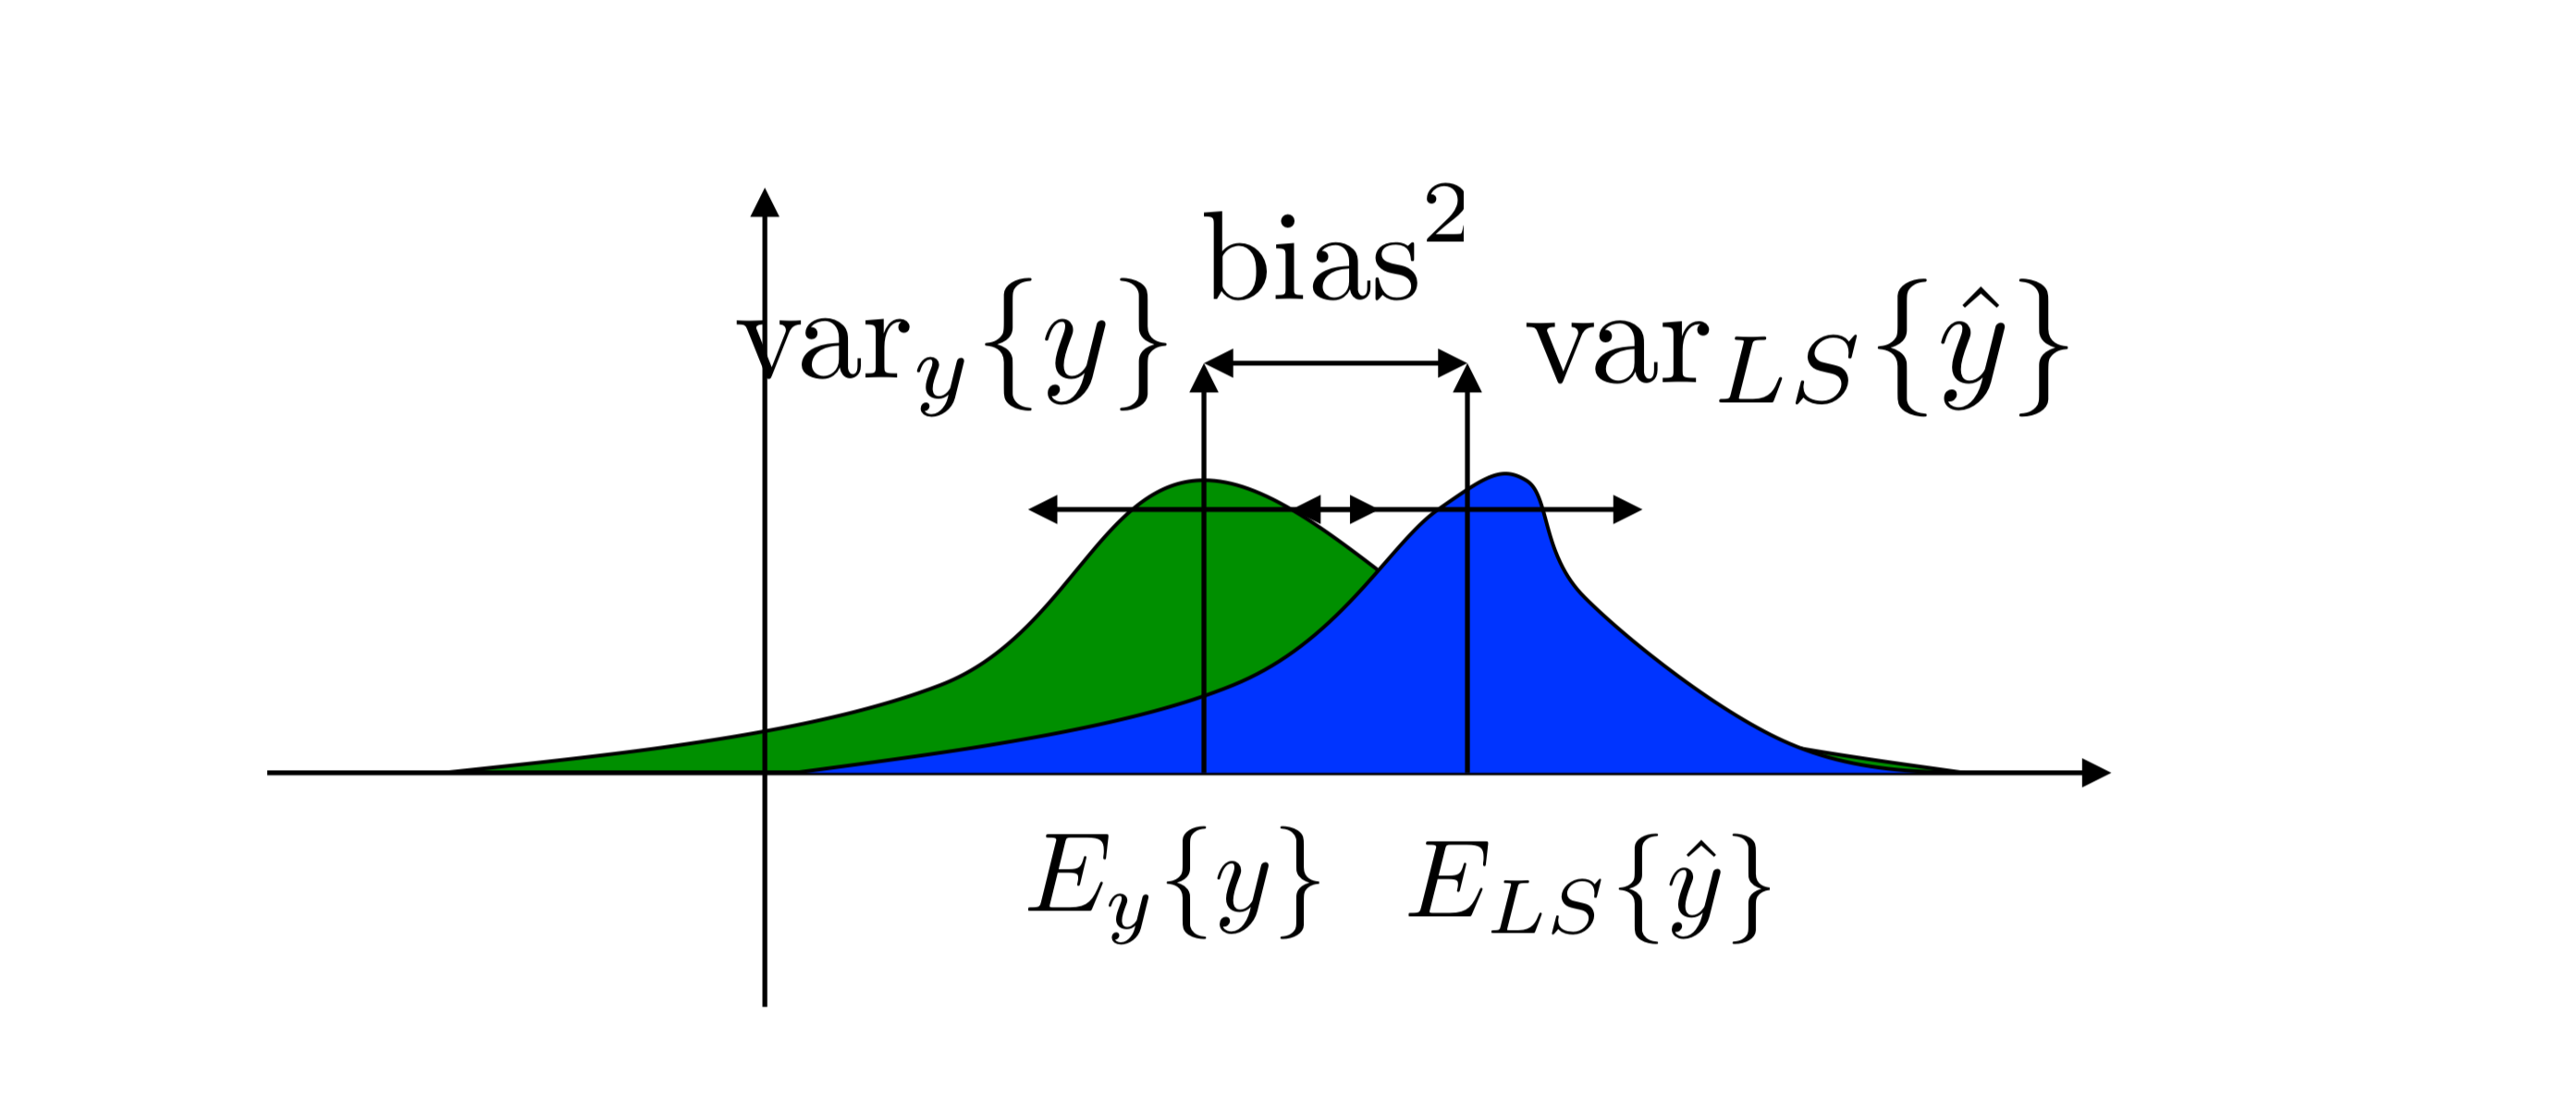
\includegraphics[scale = 0.3]{Question4/bias-variance.png}
    \caption{Caption}
    \label{fig:my_label}
\end{figure}
L'erreur mentionnée précédemment était dans le cas d'absence d'entrées.
Pour plusieurs entrées, l'erreur qu'un bon algorithme d'apprentissage devrait minimiser est:
$$E = E_{LS}\{E_{\overline{x},y}\{(y-\hat{y}(x))^2\}$$
et puisque $ E_{\overline{x},y}\{....\} = E_{\overline{x}}\{E_{y|\overline{x}}\{....\}\}$, il vient: 
$$ E = 
 \textcolor{blue}{E_{\overline{x}}\{VAR_{y|\overline{x}}\{y\}\}}
+ \textcolor{teal}{ E_{\overline{x}}\{Bias^2(\overline{x}\}}
+  \textcolor{red}{ E_{\overline{x}}\{VAR_{LS}\{\hat{y}(\overline{x}\}\} }
$$

\begin{itemize}
    \item  $\textcolor{blue}{VAR_{y|\overline{x}}\{y\}}$ is the \textbf{noise} $\rightarrow$ \textcolor{blue}{How much "y" vary from Bayes Model}.
    \item $\textcolor{teal}{ Bias^2(\overline{x})}$ $\rightarrow$ \textcolor{teal}{Measure error btw Bayes model \& average model}.
    \item $\textcolor{red}{ VAR_{LS}\{\hat{y}(\overline{x}\}}$ $\rightarrow$ \textcolor{red}{ How much "$f(\overline{x})$ "vary from one LS to another}.
\end{itemize}
\subsection{Low variance \& High Biais}
Your model is far from the bayes model (BIg error) the learning algo is giving the same model $\approx$ watever the LS $\rightarrow$ \textbf{Under-fitting}
\subsection{Low Biais \& High variance}
Your model is close to the bayes model for the objects in the LS (low error) but your model is highly dependent of your LS $\rightarrow$ \textbf{Over-fitting}
\subsection{Parameter that influence Biais \& variance}
\begin{itemize}
    \item Complexity of the Model $\nearrow$ $\Rightarrow$ \textcolor{teal}{\textbf{Biais}} $\searrow$ \&  \textcolor{red}{\textbf{variance}} $\nearrow$
    \item Complexity of Bayes model $\nearrow$ $\Rightarrow$ \textcolor{teal}{\textbf{Biais}} $\searrow$ \& no behavior of \textcolor{red}{\textbf{variance}}
    \item \textcolor{blue}{\textbf{Noise}}  $\nearrow$ \Rightarrow \textcolor{red}{\textbf{variance}} $\nearrow$  $\Rightarrow$  \textcolor{teal}{\textbf{Biais}} $\approx$ unafflected
    \item \textbf{LS} $\nearrow$ $\Rightarrow$ $\Biais$ $\approx$ unafflected and $\variance$ $\nearrow$ ($\noise$  has less impact)
\end{itemize}
Learning algo:
\begin{itemize}
    \item $\linreg$ : Hight $\Biais$ \& small $\variance$
    \item $\regtr$: Small $\Biais$ \& Hight $\variance$
    \item \textbf{knn}
    \begin{itemize}
        \item k=1: Moderate $\Biais$ \& hight $\variance$
        \item k=10: Moderate $\Biais$ \& small $\variance$
    \end{itemize}
\end{itemize}
\section{Variance Reduction technique}

First, as we know $\Biais$ and $\variance$ are inversely proportional. Reducing $\variance$ will increase the $\Biais$.\\
$\Variance$ Reduction Technique: Reduce the ability of the algorithm to fit the learning sample.
\begin{enumerate}
    \item \textbf{Prunning}: Reduce the model complexity.\\
    $\Example$: DT pruning: will try to remove sections of the tree that provide little power to classify instances.
    \item \textbf{Early stopping}: Stop the search for optimal fit to LS before reaching optimun.
    \item \textbf{Regularization}; Reduce the hypothesis space (the number of candicate models) in wich you will search.\\
    $\Example$: Neural networks weights decay $\rightarrow$ penalize height weight
    \item \textbf{Ensemble Methodes}: combine the predictions of several models buit with learning algorithms mode and order models:\\
    $\Example$: Bagging, Random Forst, Boosting, ...\\
\end{enumerate}

\section{Classification and Regression Trees}
\subsection{Classification Trees}
$\ct$ is a learning algorithm that can handle binary/Mult-value classificaiton problems with discrete Binary/Mult-value on continus attributs.\\
\textbf{Hypothesis space}:\\
A decision tree is a tree where
\begin{itemize}
    \item Each \textbf{interior nodes} test an attributes
    \item Each \textbf{branch} correspond to an attribute value
    \item Each \textbf{Leaf} node is labelled with a class
\end{itemize}

  \begin{table}[!h]
    \begin{center}
    \begin{tabular}{| m{8em}| m{30em}|}
    \hline
    \centering
    \rowcolor{blue.g} \textbf{Goal}     &  \begin{itemize}
                                              \item Choose a [trees structure/prediciton] model that \textbf{minimize} the \textbf{miss-classification} error  and \textbf{simple}  
                                          \end{itemize}\\ \hline
                                          
    \centering
    \rowcolor{vert.g} \textbf{Optimal}     &  \begin{itemize}
                                              \item Simple \& cohérent avec le LS
                                          \end{itemize}\\ \hline
                                                                                
    \end{tabular}
    \end{center}
    \end{table}

Some $\example$:
\begin{figure}[H]
    \centering
    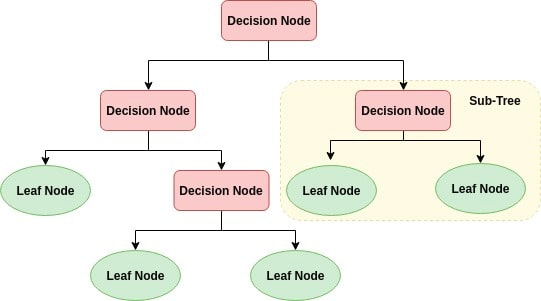
\includegraphics[scale = 0.5]{Question6/DT.jpg}
    \caption{$\Dt$ 1}
    \label{fig:my_label}
\end{figure}
\begin{figure}[H]
    \centering
    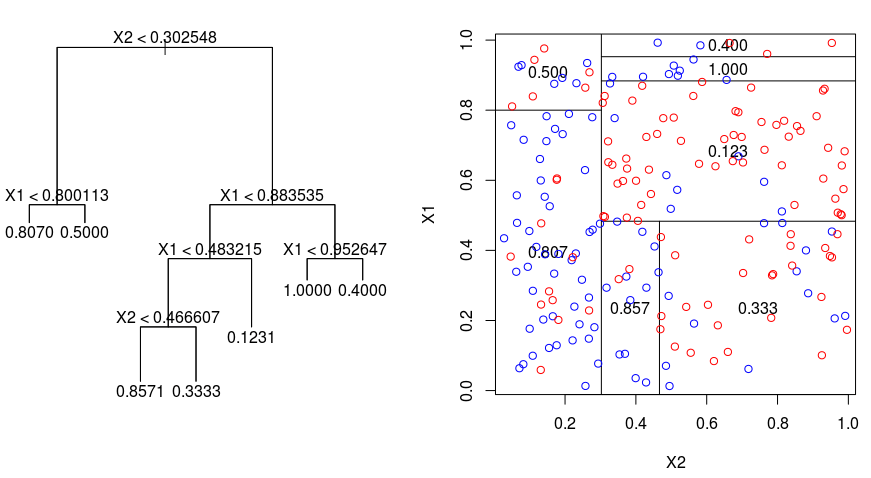
\includegraphics[scale = 0.5]{Question6/DT1.png}
    \caption{$\Dt$ 2}
    \label{fig:my_label}
\end{figure}
\begin{figure}[H]
    \centering
    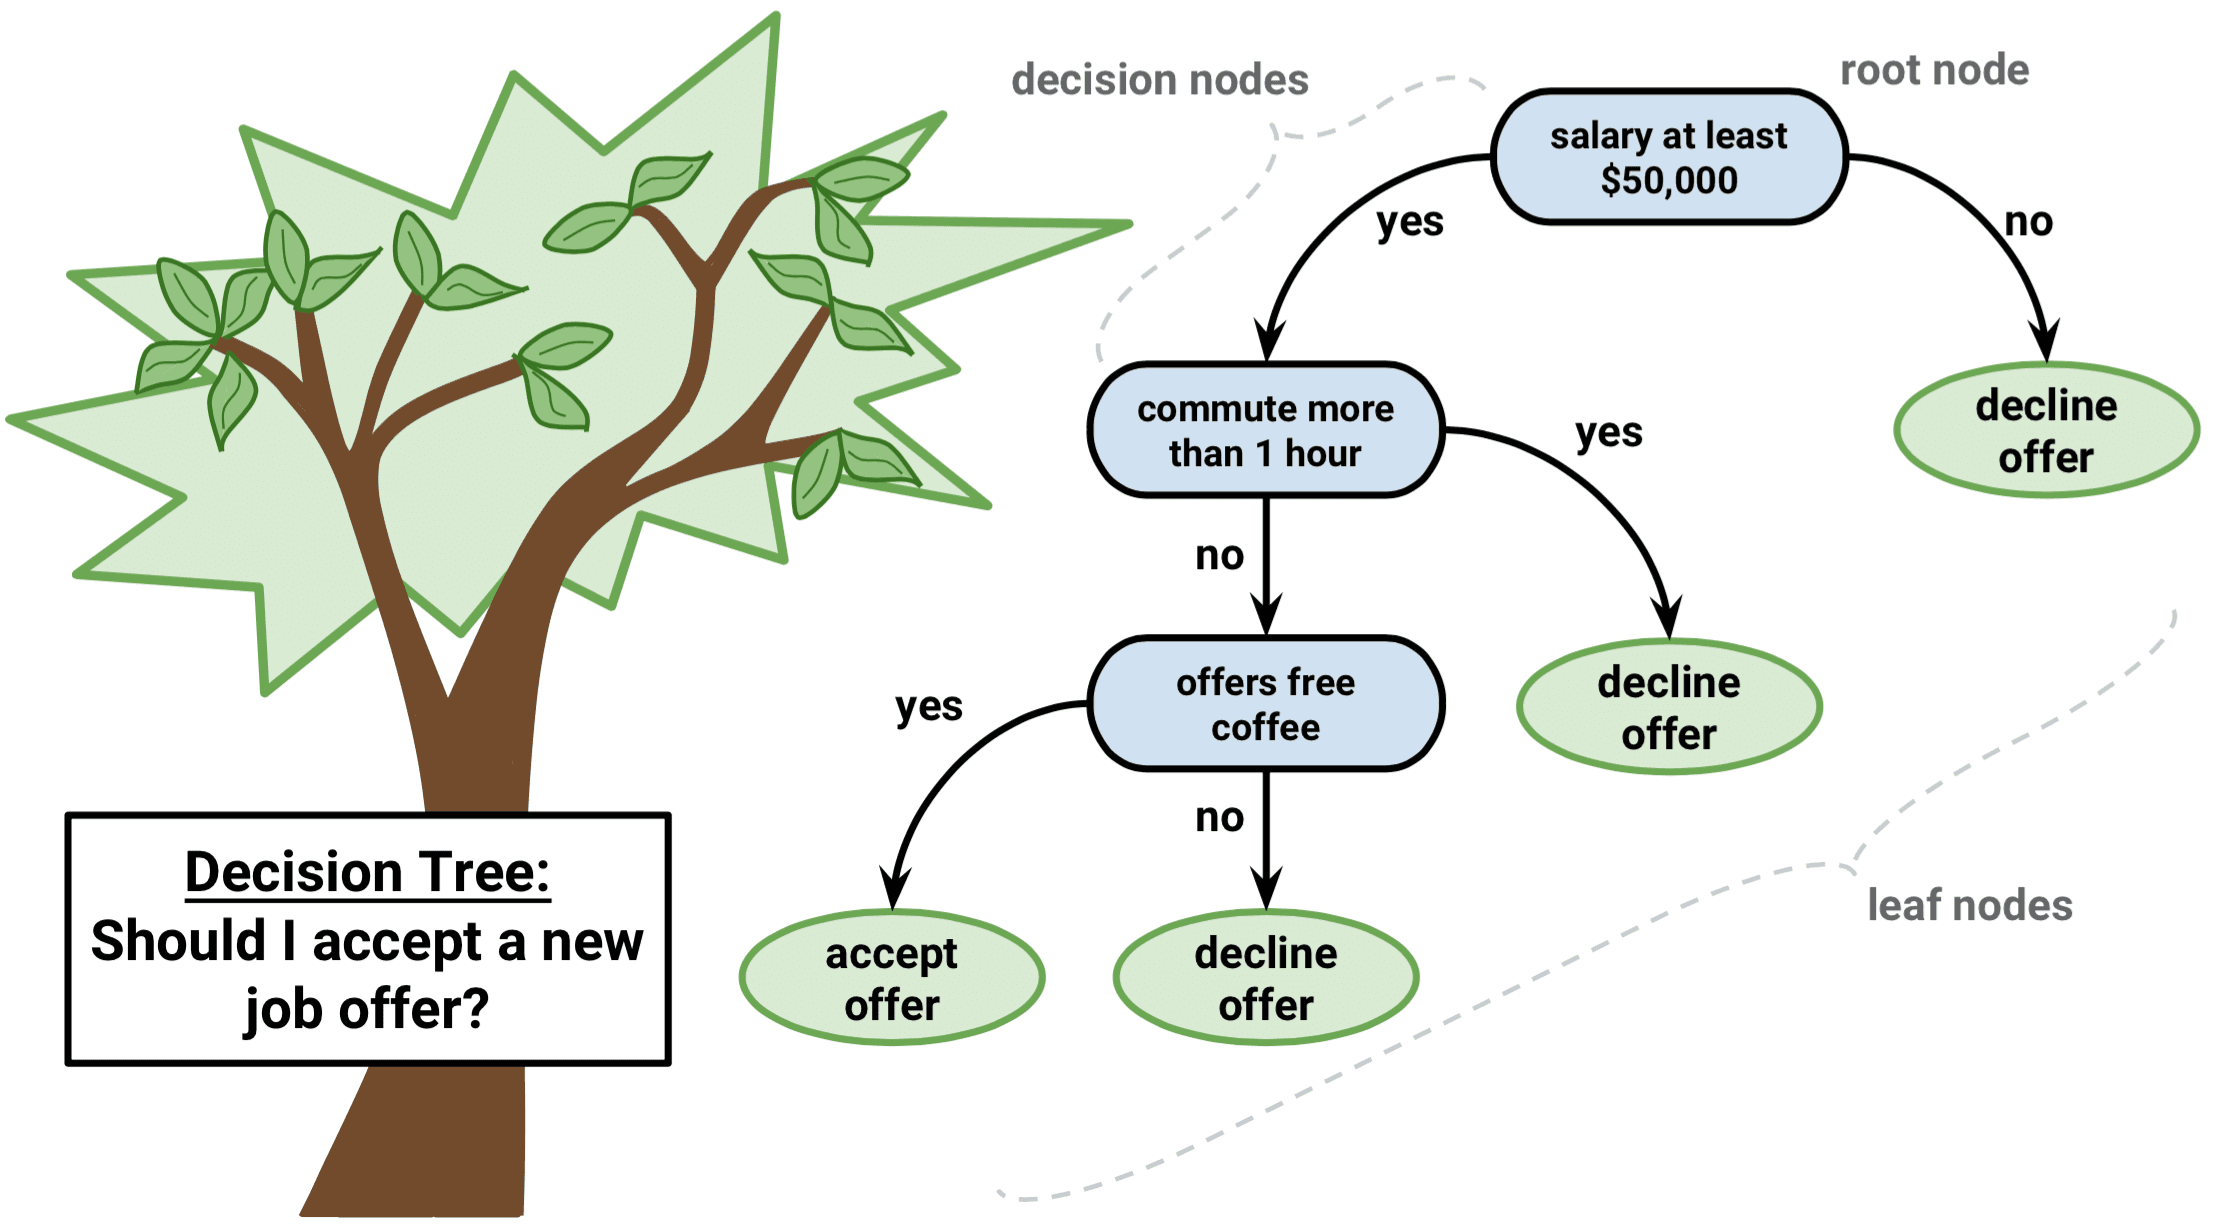
\includegraphics[scale = 0.2]{Question6/DT2.png}
    \caption{$\Dt$ 3}
    \label{fig:my_label}
\end{figure}
%---------------------------- Top-down introduction of DTs -----------------------------------
\subsection{Top-down introduction of DTs}

  \begin{table}[H]
    \begin{center}
    \begin{tabular}{| m{8em}| m{30em}|}
    \hline
    \centering
    \rowcolor{blue.g} \textbf{Method}     &  \begin{enumerate}
                                                \item Choose"Best" attribute
                                                \item Split the LS according to this attribute
                                                \item Proceed Recurcively until each object is correctely classified
                                            \end{enumerate} \\\hline    
    \centering
    \rowcolor{vert.g} \textbf{Properties}     &  \begin{enumerate}
    \item  \textbf{Fast} but \textbf{sub-optimal}
    \item Highly dependent on attribute selection criteria
    \item Hill-climbing algotithm in the space of possible $\dt$ $\rightarrow$ No backtracks \textcolor{red}{simply add sub-trees to current trees}
\end{enumerate}\\ \hline
                                                                                
    \end{tabular}
    \end{center}
    \end{table}
    
Let's define an"impurity measure" I(LS) such that
\begin{enumerate}
    \item I(LS) is \textbf{minimun} if $p_i=1 $ and $p_j=0$, $\forall i \ne j$
    \item I(LS) is \textbf{maximun} if $p_j = \frac{1}{j}$
    \item I(LS) is \textbf{symmetric} with respect to $p_1,..p_j$
\end{enumerate}
The reduction of impurity induced by a split 

  \begin{table}[H]
    \begin{center}
    \begin{tabular}{| m{8em}| m{30em}|}
    \hline
    \centering
    \rowcolor{blue.g} \textbf{Impurity}     &  \begin{itemize}
                                                \item $\Delta I(LS,A) = I(LS) - \sum_a \frac{|LS_a|}{LS}I(LS_a)$
                                                \item $\Delta I$ is the "score measure" (the quantity to \textbf{maximize})
                                                \end{itemize} \\\hline    
    \centering
     \rowcolor{vert.g} \textbf{Impurity}     &  \begin{itemize}
                                                 \item Shannon entropy
                                                 \item Gini Index
                                                 \item Missclass error rate
                                            \end{itemize} \\\hline    
                                                                                
    \end{tabular}
    \end{center}
    \end{table}
    
Used by the CART (classification and regression tree) algorithm for classification trees, Gini impurity is a measure of how often a randomly chosen element from the set would be incorrectly labeled if it was randomly labeled according to the distribution of labels in the subset. The Gini impurity can be computed by summing the probability 
$p_{i}$ of an item with label 
i being chosen times the probability 
$\sum _{k\neq i}p_{k}=1-p_{i}$ of a mistake in categorizing that item. It reaches its minimum (zero) when all cases in the node fall into a single target category.

\subsection{Pré-prunning}
Le pré-prunning stoppe la croissance de l'arbre avant qu'il ne le classifie parfaitement le LS. Arrêter de scinder un noeud si le nombre d'objets est trop petit, si l'impureté est suffisamment faible ou si le meilleur test n'est pas stastiquement significatif.\\
\textbf{Stop condiiton}:
\begin{enumerate}
    \item Nb of objects is too small to split
    \item Imputrity is low enough
\end{enumerate}

%--------------------------- post-prunning ---------------------------------------------------
\subsection{Post-pruning}

\begin{enumerate}
    \item Scinder le LS en deux: GS(growing sample) pour construire l'arbre et \textbf{VS}(calidation sample) 
    pour évaluer son erreur de généralisation. 
    \item Construire un arbre avec GS.
    \item Calculer une séquance d'arbres ${T_1,T_2,..,T_{i-1},T{i},...}$ où T\_i es obtenu en supprimant certains noeuds test de $T_{i-1}$.
    \begin{itemize}
        \item A chaque étape, supprimer le noeud qui diminue le plus l'erreur sur VS.
        \item Définir un critère de coût-complexité et construire la séquance d'arbres qui minimisent le critère.
    \end{itemize}
    \item Sélectionner le $T_i$ qui minimise l'erreur sur le \textbf{VS}
\end{enumerate}
%--------------------------- Tree sequence constructive --------------------------------
\subsection{Tree sequence constructive}
\textbf{2 methodes:}
\begin{enumerate}
    \item \textbf{Reduce error prunning}: \begin{itemize}
        \item at each step, remove the node that most decrease the error on \textbf{LS}
    \end{itemize}
    \item \textbf{Cost-complexity Prunning}
    \begin{itemize}
        \item Define Cost-complexity criteria : $$\textrm{Error}_{GS} + \alpha.\textrm{ complexity}(T)$$
        \item Build the sequence that minimizes this criteria for groing "$\alpha$"
    \end{itemize}
    \textcolor{ao}{ If small DB, use N-fold cross validation}
\end{enumerate}
%--------------------------- Continuous attributes -------------------------------------
\subsection{Continuous attributes}
\textbf{2 solutions:}

  \begin{table}[H]
    \begin{center}
    \begin{tabular}{|m{20em}|}
    \hline
    \rowcolor{blue.g} \textbf{Pre-discretation}\\ \hline
    \rowcolor{vert.g} \textbf{Discretize while tree growth}            
    \end{tabular}
    \end{center}
\end{table}


In addition to find the best attribute, you will also need to find the best cut-point where to discretize. \textcolor{red}{Use of impurity measure as well}
%--------------------------- Multi-value Attributes -------------------------------------
\subsection{Multi-value Attributes}

 2 solutions:
  \begin{table}[H]
    \begin{center}
    \begin{tabular}{|m{20em}|m{20em}|}
    \hline
    \rowcolor{blue.g} \textbf{Penalized attributes with several values} & To avoid data fragmentation too quick caused by multi-value attributes\\ \hline
    \rowcolor{vert.g} \textbf{Consider binary spits} &           
    \end{tabular}
    \end{center}
\end{table}
 But for "\textbf{N}" values attributes $\rightarrow 2^{N-1}$ possible split.\\
 \textcolor{red}{heurishcs if N  "$>>$"}

%--------------------------- Regressions TREE ----------------------------------------------
\subsection{Regression Trees}
Learning algorithm that will handle regression problems (real outputs) with real/discrete attributes.\\
\textbf{Hypothesis space}:\begin{itemize}
    \item similar to class $\dt$\\
    \textcolor{red}{but} leaf nodes are labelled whith a real NB.
\end{itemize} 

\textbf{Tree concstruction}

  \begin{table}[H]
    \begin{center}
    \begin{tabular}{|m{20em}|m{20em}|}
    \hline
    \rowcolor{blue.g} \textbf{Methods} & \begin{enumerate}
    \item Prediction at a leaf 
    \item Impurity of sample:\textbf{ $I(LS) = var_{y|LS}\{y\}$}
    \item best split: split reducing the most the $\variance$
\end{enumerate}\\ \hline
    \rowcolor{vert.g} \textbf{Prunning \algo} &    \begin{enumerate}
    \item pre-prunning : same
    \item post-prunning: use of mean squared error as quality measure
\end{enumerate}       
    \end{tabular}
    \end{center}
\end{table}


\subsubsection{Interpret ability}
DT are ofen used to pre-processed LS to avoid irrelevant varibles as it's a model with a very good/clean visualization of the relatin bwt inputs and outputs

\subsubsection{Advantages/Drawbacks}
  \begin{table}[H]
    \begin{center}
    \begin{tabular}{|m{20em}|m{20em}|}
    \hline
    \rowcolor{vert.g} \textbf{Advantages} & \begin{enumerate}
    \item Fast: $(n\log n)$ 
    \item flexible
\end{enumerate}\\ \hline
    \rowcolor{red.g} \textbf{Drawbacks} &    \begin{enumerate}
    \item Tree instability \textbf{Hight variance} (overfit quickly)
    \item not accuracy
\end{enumerate}       
    \end{tabular}
    \end{center}
\end{table}

\section{Linear regression Model}
It's a learning \algo that will: given numerical inputs,try to approximate tue output by:
\textcolor{blue}{$$\hat{y}(0) = w_0 + \sum_{i = 1}^{n} w_i \phi (a_i(0)$$}
thus, the learning \algo will need to choose the $w_0,w_1,...w_n$ parameters. So that model fot well the \textbf{LS} \textcolor{red}{and} has good generalization to unseen data objects. 

%-------------------------------------------- Least mean square error solution --------------------------------------------
\subsection{Least mean square error solution}
we will pich the set parameters minimizing the MSE.\\\\
\textcolor{blue}{\textbf{Hypothesis}}:
\begin{itemize}
    \item $a_0(0) = 1, \forall 0 \rightarrow$ \textcolor{red}{This is the "\biais value"}\\\\
    \textcolor{ao}{"$W_0$ will thus allow you to connect the \biais of the model.}
    \item $\underline{a}'(0_i)$ = (a_0(0_i), a_1(0_i), ... a_n(0_i))^T$
    \item $\underline{w}'$ = (w_0,w_1, ... w_n)^T$
\end{itemize}
Thus, we have
\textcolor{blue}{$$SE = (y(o_i)-\hat{y}{(o_i))^2 = ((y|0_i)) - \underline{w}'^T \underline{a}'(o_i))^2$$}
\textcolor{blue}{$$TSE = \sum_{i=1}^n (y(o_i)- \underline{w}'^T \underline{a}'(o_i))^2}$$}
\textcolor{blue}{$$= (\underline{y}- A'^T \underline{w}')^T(\underline{y}- A'^T \underline{w}')$$}

%------------------------------- Regularization  -------------------------------

\section{K-Nearest Neighbors}

%------------------------------------------------------- 1-NN algorithm -------------------------------------------------------
\subsection{1-NN algorithm}
\textbf{Method}: 
\begin{enumerate}
    \item you define a "\textcolor{blue}{Distance measure}" trying to infer "\textcolor{blue}{proximity}" btw object:\\
    \example : Euclidian distance 
    \textcolor{red}{$$d_a(0,0')= (a(0)-a(0)')  (a(0)-a(0'))^T = \sum_{i=1}^N(a_i(0)-a_i(0'))^2$$}
    \item you will define the "Nearest Neighbor"
    $$NN_a(LS,o) = \textrm{argmin}_{o' \in LS } d_a(0,0')$$
    \item you will extrapolate the corresponding output
    $$\hat{y}NN(o) = y(NN_a(LS,o)$$
\end{enumerate}
\textbf{Proêrties}:
\begin{enumerate}
    \item Complexity (Time)
    \begin{itemize}
        \item Fast trainsing $\rightarrow$ only storage of "LS" (n x N)
        \item Slow testing $\rightarrow$ "N" distannces computation => O(n* N)
    \end{itemize}
    \item Accuracy
    \begin{itemize}
        \item suboptimal: \textcolor{red}{Exceplt}, for det problems
        \item strong dependance on attribute choices
    \end{itemize}
\end{enumerate}
\section{From single Neurons to multilayer perceptron}
\section{Neural networks}
On peut voir chaque couche du réseau de neurone comme un vecteur:
\textcolor{blue}{$$[a_0^{(0)}+a_1^{(0)} + a_2^{(0)} + a_3^{(0)} +...+ a_n^{(0)}]^T$$}
et chaque connection entre une couche et un neuron particulier vers la couche suivant comme une matrice de poids:

$$
\begin{bmatrix}
w_{0,0} & w_{0,1} &... &w_{0,n}\\
w_{1,0} & w_{1,1} &... &w_{1,n}\\
: & :   & ^{.}. & :\\
w_{n,0} & w_{n,1} &... &w_{n,n}\\
\end{bmatrix}$$}
 Ce que cela signifie, c'est de prendre la somme pondérée des activations dans la première couche en fonction de ces poids ?
$$
\sigma
\begin{pmatrix}
\textcolor{ao}{
\begin{bmatrix}
w_{0,0} & w_{0,1} &... &w_{0,n}\\
w_{1,0} & w_{1,1} &... &w_{1,n}\\
: & :   & ^{.}. & :\\
w_{n,0} & w_{n,1} &... &w_{n,n}\\
\end{bmatrix}}
\textcolor{blue}{
\begin{bmatrix}
a_0^{(0)}  \\
a_1^{(0)}  \\
:  \\
a_n^{(0)}  \\
\end{bmatrix}}
+
\textcolor{teal}{
\begin{bmatrix}
b_0  \\
b_1  \\
:  \\
b_n  \\
\end{bmatrix}}
\end{pmatrix}
= \begin{bmatrix}
a_0^{(1)}  \\
a_1^{(1)}  \\
:  \\
a_n^{(1)}  \\
\end{bmatrix}
$$
Dés lors, des qu'on à la connaisance du vecteur \textcolor{ao}{\textbf{w}} et du \biais \textcolor{teal}{\textbf{b}} on peut trouver la valeur du neuronnes suivants:
$$a_{(1)} = \sigma(\textcolor{ao}{\textbf{W}}a^{(0)} + \textcolor{teal}{\textbf{b})}$$

\subsection{La descente de gradient, ou comment un réseau de neuronal apprend}
Remember conceptually we're thinking of each neuron as beiing connected to all of the neurons in the previous layer and the weights in the weighted sum defining its activation are kind of like the strenghs of these connection and the bias is somme indication of wheter that neuron tends to be active or inactive and to start things off. We're just gonna initialize all of those weights and biaises totally randomely needless to say this network is going to perform pretty horribly on a given trainning example since it's just doing something random for example you feed in this image of a 3 and the output layer it just lokks like mess. So what you do is you define a cost function a way of telling the computer.\\
That output should have activations which are zero for most neurons, but one for this neuron what you gave me is utter trach. To say that more mathematically what you do is add up the squares of differances between each of these trash output activation and the value that you want them to have and this what we'll call the cost of single training example.\\
botice this sum is small when the network confidantly classifies the images correctly, but it's large when the network seems like it doesn't really what it's doing.

\subsection{Radials basis function network}
A neural network with a single hidden layer with Radial basis function as activations function.

  \begin{table}[!h]
    \begin{center}
    \begin{tabular}{| m{8em}|}
    \hline
    \rowcolor{vert.g} \textbf{Faster to train than MLP}    \\\hline
    \end{tabular}
    \end{center}
    \end{table}

\begin{figure}[H]
    \centering
    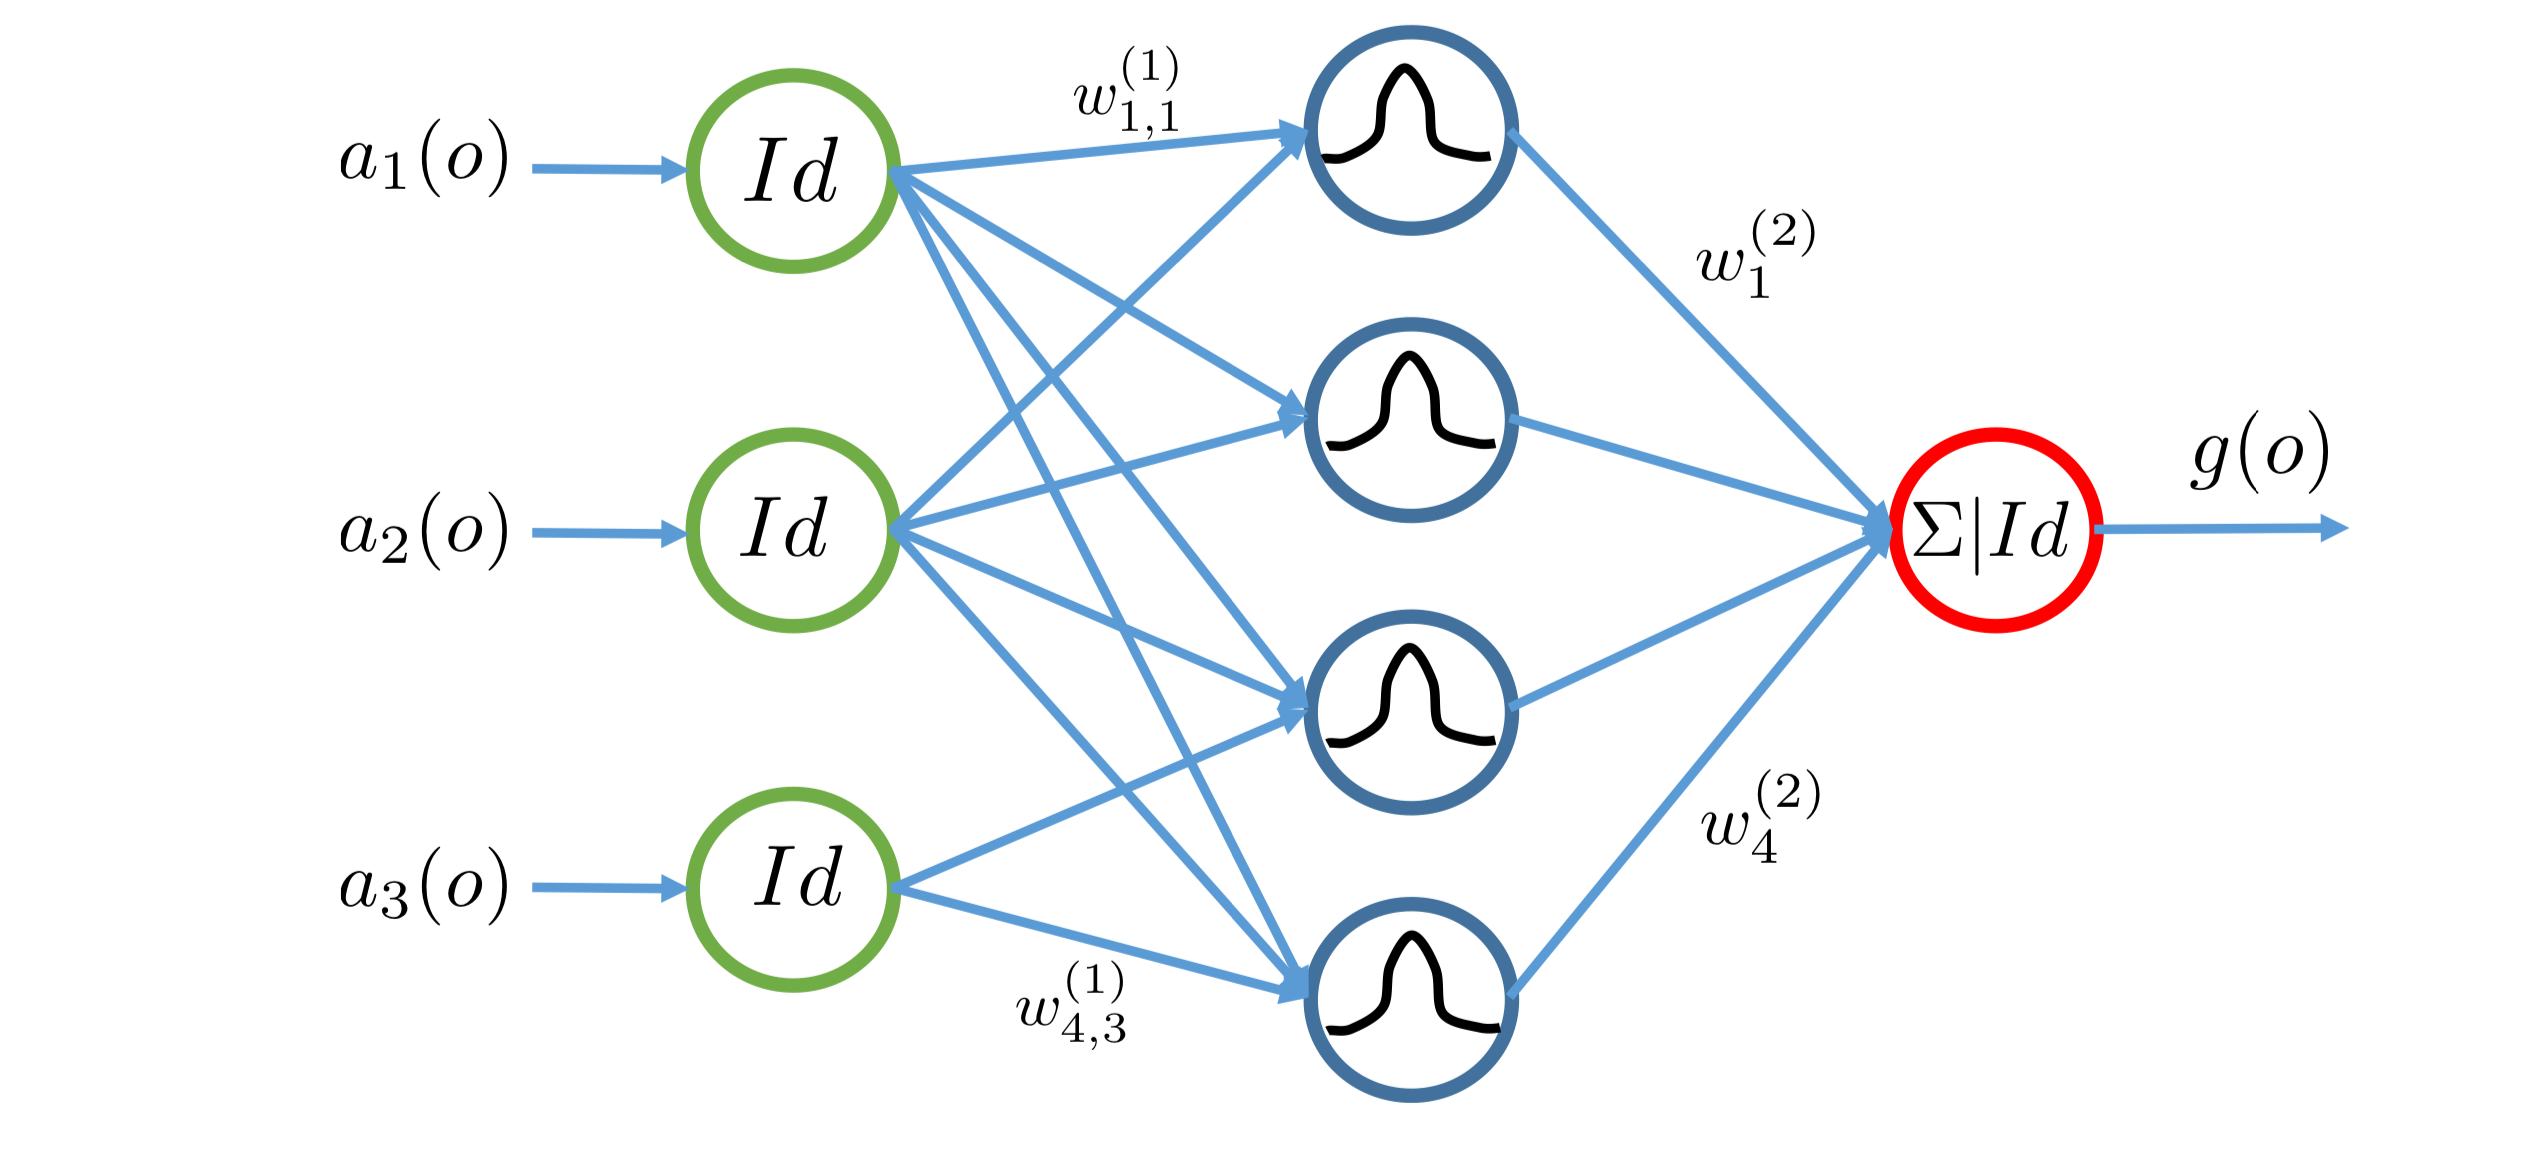
\includegraphics[scale = 0.3]{Question10/RadialBasisFunctionNetwork.png}
    \label{fig:my_label}
\end{figure}
  \subsection{Concolution NN} 
    \begin{table}[!h]
    \begin{center}
    \begin{tabular}{| m{8em}| m{15em}|}
    \hline
    \rowcolor{vert.g} \textbf{Concolutional Layer}     &  \begin{itemize}
                                                        \item Consiste of several layers where neurons are connected only to local re
                                                 \end{itemize}\\ \hline 
    \rowcolor{blue.g} \textbf{Pooling layer}       &  \begin{itemize}
                                                        \item \Each neuron is connected only to a local region (along width and height) at the same depth as its own depth in the previous layer
                                                 \end{itemize}\\ \hline
    \end{tabular}
    \end{center}
    \end{table}
    
        
    
    
        
\input{Question11/Q11.tex}
\input{Question12/Q12.tex}
\section{Ensemble Methods}
\textcolor{blue}{\textbf{Ensemble methods}} is combine the predictions of several models built with a learning algorithm in order to imrpopve with respect to the use of single model.\\
There are families methods:
\begin{enumerate}
    \item \textcolor{red}{\textbf{Averaging techniques}}: you will grow several models independently and simply average their predictions.( \textcolor{red}{\textbf{Decrease variance}})\\
    \Example : Bagging, Random Forest, ...\\
    \item  \textcolor{red}{\textbf{Boosting type algorithms}}: You grow several models sequentially.  \textcolor{red}{\textbf{Decrease \Biais}}\\
    \Example: Adaboost,...
\end{enumerate}
% -------------------------------- Bagging ----------------------------------
\subsection{Bagging}
We divide a \textbf{LS} in a sum of $\textbf{LS}_i$. Since bagging is an "\textbf{averaging techniques}", we know that the \variance must be decrease and they are no effect on the \biais.\\
So we will compute the averge model :$$\hat{y}_{ens}(\textbf{x}) = \frac{1}{T}\sum_{i=1}^{T}\hat{y}_{LS_i}(\textbf{x})$$
Since tradeoff \biais \& \variance, 
$$ E = 
 \textcolor{blue}{E_{\overline{x}}\{VAR_{y|\overline{x}}\{y\}\}}
+ \textcolor{teal}{ E_{\overline{x}}\{Bias^2(\overline{x}\}}
+  \textcolor{red}{ E_{\overline{x}}\{VAR_{LS}\{\hat{y}(\overline{x}\}\} }
$$
we can do maths:
\begin{itemize}
    \item The \biais : 
    $ \textcolor{teal}{ E_{\underline{x}}\{E_{y|x}\{y\}\}- \{E_{LS}\{\hat{y}_{ens}\{\underline{x}\}\}} $
    \begin{itemize}
        \item $ \textcolor{teal}{\{E_{y|x}\{y\}\}}$ remains unchanged (Bayes model)
        \item  $ \textcolor{teal}{E_{LS}\{\hat{y}_{ens}\{\underline{x}\}}
        = {E_{LS}\{\frac{1}{T}\sum_{i=1}^{T}\hat{y}_{LS_i}(\textbf{x})\} = {E_{LS}\{\hat{y}_{LS}(\underline{x})\} $, also remains unchanged
    \end{itemize}
    \item The \variance :  $ \textcolor{red}{ E_{\underline{x}}\{E_{LS}\{(\hat{y}_{ens}\{\underline{x}\}- \{E_{LS}\{\hat{y}_{ens}\{\underline{x}\}\})^2\}} $
     \begin{itemize}
        \item $ \textcolor{red}{E_{LS}\{(\frac{1}{T}\sum_{i=1}^{T}\hat{y}_{LS_i}(\textbf{x})- \{E_{LS}\{\frac{1}{T}\sum_{i=1}^{T}\hat{y}_{LS_i}(\textbf{x})\}\})^2\}} $\\
        \item As we can seen, the fist part of the obove equation, devide the \variance per T
    \end{itemize}
    
\end{itemize}
\textbf{But} in practice, we can not draw several \textbf{LS} because proba distribution is unkknown. \textcolor{blue}{Use of "\textbf{Boostmap sampling}"}
% -------------------------------- Random Forest ----------------------------------
\subsection{Random Forest}
\textbf{Random forest} = \textbf{Bagging} + \textbf{Random attribtute subset selection}
\begin{enumerate}
    \item Build the tree from \textbf{Boostmap sample}
    \item Instead of choosing best split among all a attributes
\end{enumerate}
% -------------------------------- Boosting ---------------------------------------
\subsection{Boosting}
you will try to compute the \textbf{outputs} of many "weaks"\textcolor{ae}{(Model with high biais, slightly better than random guess for class}. Models to produce a powerfull ensemble of methods.
% -------------------------------- Stoching ---------------------------------------
\subsection{Stoching}
\section{Feature selection}
\textbf{Goal}: reduce the number of features used by the learning algorithm on order to: \begin{enumerate}
    \item Avoid overfiiting (eviter l'overfiiting): \textcolor{ae}{some feature might be "irrelevant" for the problem}, \textcolor{red}{fittingthem = overfitting}}
    \item Improve interpretability 
    \item provide faster and more cost-eff model
    \item reduce computing time: ⚠  if fast feature selection
\end{enumerate}

There are two type of feature selection techniques.
\begin{enumerate}
    \item \textbf{Features selection} : Find a small or smallest subset of features that maximize accuracy.
    \item \textbf{Features ranking}: sort the varibles according to ther relevance at predicting output. 
\end{enumerate}

\subsection{Filter techniques}
Filter techniques is a priori selection of the varibles. Independent of learning algo.
\textbf{Method}\begin{enumerate}
    \item Associate a relevance score to cach variable : "Score explained"
    \item Remove low-scoring Features \textcolor{ao}{Treshold neeeded}
\end{enumerate}
There are two type of "\textbf{scoring}"
\begin{enumerate}
    \item \textbf{Univariate scoring}: score each feature independdently. \Example stat test (t-test,..)
    \item \textbf{Multivariate scoring}: score features dependently. Some features are useless alone \textbf{But} with others they perfectly representthe LS. 
\end{enumerate}




  \begin{table}[!h]
    \begin{center}
    \begin{tabular}{| m{8em}| m{25em}|}
    \hline
    \rowcolor{vert.g} \textbf{Advantages}     &  \begin{itemize}
    \item Univariate fitten tech : \textbf{Fast \& scalable}
    \item independent of the learning \algo
\end{itemize}\\ \hline 
    \rowcolor{red.g} \textbf{Drawbacks}       &  \begin{itemize}
    \item Independant of te learning algo: can't be totally efficient.
    \item Univariate: Ignore feature dependecie.
    \item Multivariate: \textbf{slower} than univariate.
\end{itemize}\\ \hline
    \end{tabular}
    \end{center}
    \end{table}



\Example Multivariate scoring: Decision Trees,...
%--------------------------------- Embedded Techniques --------------------------
\subsection{Embedded Techniques}
Some learning algorithms embedded some feature selection: \textbf{Search for an optimal subset} of features is build into the LS.\\
\Example:
\begin{enumerate}
    \item Decision tree node spliting: feature selection techninques 
    \item Weight in svm Model
\end{enumerate}



  \begin{table}[!h]
    \begin{center}
    \begin{tabular}{| m{8em}| m{25em}|}
    \hline
    \rowcolor{vert.g} \textbf{Advantages}     &  \begin{itemize}
    \item computationnaly efficient. 
    \item Well integrated in the learning \algo 
    \item Multivarite 
\end{itemize}\\ \hline 
    \rowcolor{red.g} \textbf{Drawbacks}       &  \begin{itemize}
    \item learning \algo specific
\end{itemize}\\ \hline
    \end{tabular}
    \end{center}
    \end{table}

%--------------------------------- wappen technique --------------------------
\subsection{wappen technique}
Find a subset of features that maximizes the "\textbf{quality of the model"induced by the learning algorithm}


%--------------------------------- Selection Biais --------------------------

% ------------------------------ Selection biais ------------------------------
\subsection{Selection \biais}
\textbf{Protocol}:
\begin{enumerate}
    \item Divide LS into 10 folds
    \item  For i = 1 to 10: 
    \begin{enumerate}
        \item Remove the $i^{th}$ fold from LS $\to LS_i$
        \item select top 20 variables from LS
        \item learn model using the 20 varibles on LS 
        \item Test model on the $i^{th}$ fold 
    \end{enumerate}
\end{enumerate}
\section{Clustering Methods}
Unsupervised learning: Try to find any regularities in a dataset without any guidance about inputs or outputs. there are 3 families of problems. 
\begin{itemize}
    \item \textbf{Clustering}: Find a natural groups of sample\varibles
    \begin{enumerate}
        \item \textbf{Clustering rows} : groups similar obs. 
        \item \textbf{Clustering coloùns}:groups similar var. 
        \item \textbf{Bi-clustering} on two-way clustering: group objects that are similar considering a subset of varibles.
    \end{enumerate}
    \item \textbf{Dimentionnaly reduction}
    \item \textbf{Density estimation} : Determine the distribution of data cithin the input space
\end{itemize}
When we use the \textbf{clustering analysis}, there are \textbf{two} components:
\begin{itemize}
    \item \textbf{Distance measure}: similarity/Distance between two objects ao attributes
    \item \textbf{Clustering algotithms} : Produce to minimize distance of objects within groups and/or maximize distances between groups.
\end{itemize}

\subsection{Distance Measure}
Similarities bwt objects or attributes. Let's introduce two vector (\textbf{a},\textbf{b})
\begin{itemize}
    \item \textbf{Euclidian distance}: $d_E (\textbf{a},\textbf{b}) = \sqrt{\sum_i (a_i - b_i})^2}$ \textcolor{ao}{(Measure average difference between elements)}
    \item \textbf{Manhattan distance}: $d_m (\textbf{a},\textbf{b}) = \sum_i |a_i - b_i|$ \textcolor{ao}{(Measure vaerage difference between elements in a "\textbf{robust way}")}
    \item \textbf{Correlation distance}  : $d_C (\textbf{a},\textbf{b}) = 1- p $ \textcolor{ao}{(Measure difference with respect to trends)}
    \begin{itemize}
        \item "p" is the Pearson correlation of two vectors.
    \end{itemize}
\end{itemize}
\section{Dimentionality reduction
\subsection{PCA}
\textcolor{red}{\textbf{Limitaations}}: PCA only for a priori determined group 

\appendix
\begin{appendices}
\section{Definition}
\subsection{\textcolor{red}{Decision tree prunning}}
\textbf{Pruning} is a technique in machine learning and search algorithms that reduces the size of decision trees by removing sections of the tree that provide little power to classify instances. Pruning reduces the complexity of the final classifier, and hence improves predictive accuracy by the reduction of overfitting.
\subsection{\textcolor{red}{Impurity}}
l'impureté de Gini est une mesure de la fréquence à laquelle un élément choisi au hasard dans l'ensemble serait incorrectement étiqueté s'il était étiqueté au hasard selon la distribution des étiquettes dans le sous-ensemble. 

\subsection{\textcolor{red}{entropie de Shannon}}
L'entropie de Shannon, due à Claude Shannon, est une fonction mathématique qui, intuitivement, correspond à la quantité d'information contenue ou délivrée par une source d'information. Cette source peut être un texte écrit dans une langue donnée, un signal électrique ou encore un fichier informatique quelconque (collection d'octets).
Du point de vue d'un récepteur, plus la source émet d'informations différentes, plus l'entropie (ou incertitude sur ce que la source émet) est grande. Ainsi, si une source envoie toujours le même symbole, par exemple la lettre 'a', alors son entropie est nulle, c'est-à-dire minimale. En effet, un récepteur qui connaît seulement les statistiques de transmission de la source est assuré que le prochain symbole sera un 'a'. Par contre, si la source envoie un 'a' la moitié du temps et un 'b' l'autre moitié, le récepteur est incertain de la prochaine lettre à recevoir. L'entropie de la source dans ce cas est donc non nulle (positive) et représente quantitativement l'incertitude qui règne sur l'information émanant de la source. L'entropie indique alors la quantité d'information nécessaire pour que le récepteur puisse déterminer sans ambiguïté ce que la source a transmis. Plus le récepteur reçoit d'information sur le message transmis, plus l'entropie (incertitude) vis-à-vis de ce message décroît. En particulier, plus la source est redondante, moins elle contient d'information. En l'absence de contraintes particulières, l'entropie est maximale pour une source dont tous les symboles sont équiprobables.
\subsection{\textcolor{red}{Prunning Algorithm}}
\textbf{English}: Pruning is a technique in machine learning and search algorithms that reduces the size of decision trees by removing sections of the tree that provide little power to classify instances. Pruning reduces the complexity of the final classifier, and hence improves predictive accuracy by the reduction of overfitting.\\\\
\textbf{French}: Le Prunning est une technique de machine learning et d'algorithmes de recherche qui réduit la taille des arbres décisionnels en supprimant les sections de l'arbre qui fournissent peu de puissance pour classer les instances. Le prunning réduit la complexité du classificateur final, et améliore donc la précision prédictive en réduisant l'over-fitting.

\subsection{\textcolor{red}{Bagging}}
Le mot \textbf{Bagging} est une contraction de \textbf{Bootstrap Aggregation}. Le bagging est une technique utilisée pour améliorer la classification notamment celle des arbres de décision, considérés comme des « classifieurs faibles », c’est-à-dire à peine plus efficaces qu’une classification aléatoire.\\

En général, le \textbf{bagging} a pour but de réduire la $\variance$ de l’estimateur, en d’autres termes de corriger l’instabilité des arbres de décision (le fait que de petites modifications dans l’ensemble d’apprentissage entraînent des arbres très différents). Pour ce faire,  le principe du bootstrap est de créer de « nouveaux échantillons » par tirage au hasard dans l’ancien échantillon, avec remise. L’algorithme, par exemple l’arbre de décision, est entraîné sur ces sous-ensembles de données. Les estimateurs ainsi obtenus sont moyennés (lorsque les données sont quantitatives, cas d’un arbre de régression) ou utilisés pour un « vote » à la majorité (pour des données qualitatives, cas d’un arbre de classification).  C’est la combinaison de ces multiples estimateurs « indépendants » qui permet de réduire la variance. Toutefois, chaque estimateur est entrainé avec moins de données. En pratique, la méthode de bagging donne d’excellents résultats (notamment sur les arbres de décision utilisés en « forêts aléatoires »).

\subsection{\textcolor{red}{Clustering}}
Group a collection of objects into substeds. The "\textbf{clusters}" such that citin cach clusters data are more related to one another than objects assigned to diiferent clusters.

\subsection{\textcolor{red}{L'impurité de gini}}
L'impureté de Gini est une mesure de la fréquence à laquelle un élément choisi au hasard dans l'ensemble serait incorrectement étiqueté s'il était étiqueté au hasard selon la distribution des étiquettes dans le sous-ensemble. L'impureté de Gini est limitée par 0, 0 se produisant si l'ensemble de données ne contient qu'une seule classe. 

%--------------------------- Boosting---------------------------------------------------
\subsection{\textcolor{red}{Le boosting}}
le \textbf{Boosting} est une méthode adaptative de correction de l'erreur. A chaque étape, on à la construction d'un modèle se basant sur le modèle précedant, on en calcule l'erreur.L'idée est donc de combiner beaucoup de modèles qui sous-évaluent les données pour produire un modèle plus puissant.

%--------------------------- Extra tree ---------------------------------------------------
\subsection{\textcolor{red}{L'extra trees}}
\textbf{L'extra trees} consiste a construire un ensemble d'arbre complétement développé indépendamment généré dans lesquelles le choix des attributs des noeuds internes se fait de manière aléatoire. Pour K et $n\_{min}$ donné, à chaque étape, on prend un ensemble de K attributs dont on défini $t_i = a_{i_c} \in ]min(a_i); mac(a_i)]$ et on en garde que celui maximisant le score. On considère que le noeud est une feuille si $|S| < n_{min}$ ou que tous les attributs ou la sortie sont constant dans S. Agrégation des arbres: par moyenne des sorties (régression) ou par majorité de vote (classificaiton).\\
Cette méthode permet également lka réduction de la variance sans trop augmenter le biais.
\end{appendices}




\end{document} 
